\section{Optimizando}
\subsection{Pools en PHP}
La configuración por defecto de PHP no suele ser la óptima, dependiendo
de nuestras necesidades  y hardware deberemos ajustar algunos parámetros. En esta sección
nos centraremos en el número de procesos y recursos que se dedicarán a una
aplicación web. Estos parámetros se encuentran en el directorio \emph{/etc/php/fpm/pools.d},
se debe tener una archivo por cada aplicación, en nuestro caso será \emph{www.conf}.
Los parámetros a ajustar son:
\begin{itemize}
    \item pm: Decide cómo el controlador de procesos administra los procesos
    hijos, es recomendable establecerlo a dinámico.
    \item pm.max\_children: Cuando pm es estático, el número de hijos a crear,
    cuando es dinámico, el máximo número de hijos que se podrán tener.
    \item pm.start\_servers: Número de hijos a crear al inicio.
    \item pm.min\_spare\_servers: El número mínimo de procesos libres (Sin
    hacer nada).
    \item pm.max\_spare\_servers: Número máximo de procesos libres.
    \item pm.max\_requests: El número de peticiones que cada hijo aceptará
    antes de reiniciarse, útil para evitar pérdidas de memoria.
\end{itemize}
Hay varias aproximaciones para determinar el valor adecuado de estos parámetros,
en esta guía se verán 3, y todas con \emph{pm = dynamic}.

El primero (\cite{pools1}) consiste en calcular \emph{pm.max\_children} basándonos en
la fórmula:
\begin{equation}
    pm.max\_children = (RAM_{total} - RAM_{resto Proc})/ RAM_{mediaPHP}
\end{equation}
Donde $RAM_{resto Proc}$ es la memoria usada por los otros procesos y $RAM_{mediaPHP}$
es la media de memoria usada por los procesos de PHP. La memoria consumida
por el resto de procesos se puede calcular mediante este comando:
\begin{bashcode}
ps -ylA --sort:rss | grep -v php5-fpm |
awk '!/RSS/ { s+=$8 } END { printf "%s\n", "Memoria total usada por otros procesos"; printf "%dM\n", s/1024 }'
\end{bashcode}
Y la consumida por PHP:
\begin{bashcode}
ps -ylC php5-fpm --sort:rss  |
awk '!/RSS/ { s+=$8 } END { printf "%s\n", "Memoria consumida por PHP: "; printf "%dM\n", s/1024 }'
\end{bashcode}
Al número anterior lo dividimos por los procesos de PHP y obtenemos la media.

Una vez calculado el valor de \emph{max\_children}, \emph{min\_spare\_servers} y
\emph{max\_spare\_servers}  se suelen calcular evaluando el rendimiento y \emph{start\_servers},
suele ser:
\begin{equation}
    start\_servers = min\_spare\_servers + (max\_spare\_servers - min\_spare\_servers) / 2
\end{equation}

El segundo método (\cite{pools2}) es calcularlo en base a :
\begin{equation}
    pm.max\_children = RAM_{total} / RAM_{maxPHP}
\end{equation}
Donde $RAM_{maxPHP}$ es el process PHP que ocupe más memoria. El resto de
parámetros se calculan en base a éste.
Por último, otro método (\cite{pools3}) es realizando la operación siguiente:
\begin{equation}
    pm.max\_children = 1.2 \cdot RAM_{total}/RAM_{mediaPHP}
\end{equation}

\subsection{Optimizando Nginx} % Descartar si sobra
FastCGI es un protocolo que hace de interfaz entre programas y servidores web.
En esta sección veremos cómo configurar nginx para cachear páginas y aumentar
su rendimiento.

Para aprovechar todos los núcleos de un procesador, nginx necesita ajustar
el parámetro \emph{worker\_processes} acorde al número de procesadores. Para
determinar el número de procesadores podemos ejecutar el siguiente comando:
\begin{bashcode}
cat /proc/cpuinfo| grep processor | wc -l
\end{bashcode}
En la directiva \emph{worker\_connections} dentro del bloque \emph{events} escribiremos
un 1024. Con esto nginx tendrá un proceso por núcleo y cada proceso podrá procesar hasta
1024 conexiones.

Estableceremos ahora los parámetros que permitirán cachear los resultados
para servirlos más rápido al cliente, para ello haremos uso de las directivas
\emph{fastcgi\_cache}. En el bloque \emph{http} necesitaremos:
\begin{bashcode}
fastcgi_cache_path /var/cache/nginx levels=1:2 keys_zone=microcache:500m max_size=1000m inactive=60m;
fastcgi_cache_key "$scheme$request_method$host$request_uri";
fastcgi_cache_use_stale updating error timeout invalid_header http_500;
\end{bashcode}
Lo cual establece el directorio donde se guardarán los objetos cacheados,
los niveles de cache, un nombre y el espacio reservado (500Mb), así como
un tope máximo (1Gb). La segunda directiva establece bajo qué nombre se
almacenará la clave para la cache. Por último la tercera servirá contenido
antiguo en la caché cuando haya errores en el servidor web, cuando se esté
actualizando la caché, cuando haya errores del tipo 5xx o cuando la cabecera
de la petición sea inválida.

El siguiente paso es decidir qué objetos se almacenarán en caché y cuales no.
Para ello, dentro de un bloque \emph{server} escribiremos:
\begin{bashcode}
    set $no_cache 0;
    if ($request_method = POST) { set $no_cache 1; }
    if ($query_string != "") { set $no_cache 1; }
    location ~ \.php$ {
    # ....
    fastcgi_cache_bypass $no_cache;
    fastcgi_no_cache $no_cache;
    fastcgi_cache microcache;
    fastcgi_cache_valid 60m;
}
\end{bashcode}
En esta porción de código hemos declarado una variable que determinará qué
peticiones se cachean y cuales no. No cachearemos ninguna petición POST ni
nada que tenga consultas en la URL (?arg...\&arg1...). Con ayuda de esta variable
podremos decidir en el bloque \emph{location} si cacheamos la petición (directivas
bypass y no\_cache), aquí hacemos referencia al nombre que dimos anteriormente
al espacio de caché y fijamos un periodo de validez.
\subsection{PageSpeed}
En esta sección veremos cómo compilar y configurar el módulo desarrollado
por Google que optimizará al máximo todos los recursos de nuestra web, minimizando
considerablemente el tiempo de respuesta y aplicando algunos cambios a los
archivos para que cumplan con los estándares de rendimiento que Google usa
para puntuar las páginas web.

Algunas de las características que  ofrece son comprimir los archivos CSS y
JavaScript de forma que ocupen lo menos posible. Unificar (cuando sea posible)
la mayor cantidad de archivos CSS y JS en uno solo para reducir el número
de peticiones al servidor. Optimizar las imágenes para reducir su tamaño. Cargar
de forma asíncrona los programas JS. Mover los elementos bloqueantes que impiden
que la página se renderize correctamente a lugares donde no sean perjudiciales
para el renderizado. Éstas son solo algunas de las funcionalidades principales.

\subsubsection{Preparando el entorno}
Antes de poder compilar, será necesario instalar algunas dependencias:
\begin{bashcode}
apt-get install build-essential zlib1g-dev libpcre3 libpcre3-dev
\end{bashcode}
Una vez hecho, estamos en condiciones para descargar y compilar:
\begin{bashcode}
cd ~
wget https://github.com/pagespeed/ngx_pagespeed/archive/v1.7.30.1-beta.zip
unzip v1.7.30.1-beta.zip # or unzip v1.7.30.1-beta
cd ngx_pagespeed-1.7.30.1-beta/
wget https://dl.google.com/dl/page-speed/psol/1.7.30.1.tar.gz
tar -xzvf 1.7.30.1.tar.gz
\end{bashcode}
Hecho esto, será necesario recompilar nginx con este módulo, como comentamos
al inicio de esta guía, para ello simplemente ejecutamos:
\subsubsection{Añadir el módulo a nginx}
\begin{bashcode}
nginx -V # Para ver con qué módulos está compilado el ejecutable actual
configure arguments: --with-http_gzip_static_module --sbin-path=/usr/local/sbin --with-http_ssl_module
--without-mail_pop3_module --without-mail_imap_module --without-mail_smtp_module --with-http_stub_status_module
--with-http_realip_module
cd ~/nginx-1.4.4/ # compilaremos nginx con el nuevo módulo (--ad-module)
./configure --with-http_gzip_static_module --sbin-path=/usr/local/sbin --with-http_ssl_module
--without-mail_pop3_module --without-mail_imap_module --without-mail_smtp_module --with-http_stub_status_module
--with-http_realip_module --add-module=$HOME/ngx_pagespeed-1.7.30.1-beta
make -j 4 # compilamos
service nginx destroy # detenemos la instancia actual de nginx
make install # instalamos la nueva versión con pagespeed
\end{bashcode}
\subsubsection{Configurando PageSpeed}
Solo resta configurar nginx para activar \emph{pagespeed} con los filtros deseados.
La documentación se puede encontrar en \cite{pgspeed}. Por defecto  los filtros
habilitados son:
\begin{bashcode}
add_head
combine_css
combine_javascript
convert_meta_tags
extend_cache
fallback_rewrite_css_urls
flatten_css_imports
inline_css
inline_import_to_link
inline_javascript
rewrite_css
rewrite_images
rewrite_javascript
rewrite_style_attributes_with_url
\end{bashcode}
Veamos cómo habilitar pagespeed en nginx, para ello crearemos un fichero
y un directorio en \emph{/usr/local/nginx/conf/global/pagespeed.conf} conteniendo:
\begin{bashcode}
pagespeed on;

# Needs to exist and be writable by nginx.
pagespeed FileCachePath /var/ngx_pagespeed_cache;

# Ensure requests for pagespeed optimized resources go to the pagespeed handler
# and no extraneous headers get set.
location ~ "\.pagespeed\.([a-z]\.)?[a-z]{2}\.[^.]{10}\.[^.]+" {
      add_header "" "";
}
location ~ "^/ngx_pagespeed_static/" { }
location ~ "^/ngx_pagespeed_beacon$" { }

# This page shows statistics about the ngx_pagespeed module.
location /ngx_pagespeed_statistics {
    allow 127.0.0.1;
    allow TuIP;
    deny all;
}

# Recent log messages. Like statistics, these are generally not to be shown
# to the public, so this has access controls as well.
pagespeed MessageBufferSize 100000;
location /ngx_pagespeed_message {
    allow 127.0.0.1;
#    allow TuIP;
    deny all;
}

# This page lets you view a graphical console displaying statistics about
# the ngx_pagespeed module.  As with statistics and messages, you may
# want access control.
pagespeed Statistics on;
pagespeed StatisticsLogging on;
pagespeed LogDir /var/log/pagespeed;
pagespeed StatisticsLoggingIntervalMs 60000;
pagespeed StatisticsLoggingMaxFileSizeKb 1024;
location /pagespeed_console {
    allow 127.0.0.1;
#    allow TuIP;
    deny all;
}

# Honoring no-transform Cache-Control Headers
pagespeed DisableRewriteOnNoTransform off;
pagespeed RewriteLevel CoreFilters;

# Specifying the value for the PageSpeed header
pagespeed XHeaderValue "Gracias a ngx_pagespeed";
\end{bashcode}
Esto debería ser suficiente para la mayoría de webs, es posible habilitar
más filtros usando la directiva \emph{pagespeed EnableFilters}.

Por último hay que añadir la configuración a nginx, dentro del bloque \emph{sever}
que deseemos incluimos la línea \emph{include global/pagespeed.conf;} y
recargamos la configuración de nginx:
\begin{bashcode}
service nginx reload
\end{bashcode}
Podemos comprobar que todo funciona correctamente ojeando  las cabeceras
de la respuesta del servidor como se muestra en la figura~\ref{pagespeed}
\begin{figure}[H]
\centering
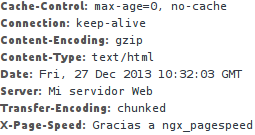
\includegraphics[scale=.5]{./img/pagespeed.png}
\caption{Comprobando la cabecera HTTP Server:}
\label{pagespeed}
\end{figure}
Como vemos, la cabecera de pagespeed está presente, luego está habilitado.
\subsection{APC}
APC viene de Alternative PHP Cache y es un opcode libre y gratuito para PHP.
Su objetivo es proporcionar un marco robusto, libre y abierto para optimizar código
intermedio de PHP mediante su almacenamiento en caché.
\subsubsection{Instalando y configurando APC}
Para instalarlo basta con ejecutar:
\begin{bashcode}
apt-get install php-apc
\end{bashcode}
El archivo de configuración reside en \emph{/etc/php5/fpm/conf.d/apc.ini}, un ejemplo de
configuración es el siguiente:
\begin{bashcode}
apc.enabled=1
apc.shm_segments=1
apc.shm_size=128M
;Relative to the number of cached files (you may need to watch your stats for a day or two to find out a good number)
apc.num_files_hint=768

;Relative to the size of your site
apc.user_entries_hint=4096

;The number of seconds a cache entry is allowed to idle in a slot before APC dumps the cache
apc.ttl=7200
apc.user_ttl=7200
apc.gc_ttl=3600

;Setting this to 0 will give you the best performance, as APC will
;not have to check the IO for changes. However, you must clear
;the APC cache to recompile already cached files. If you are still
;developing, updating your site daily in WP-ADMIN, and running W3TC
;set this to 1
apc.stat=0

;;This MUST be 0, WP can have errors otherwise!
apc.include_once_override=0

;Only set to 1 while debugging
apc.enable_cli=0

;Allow 2 seconds after a file is created before it is cached to prevent users from seeing half-written/weird pages
apc.file_update_protection=2

;Leave at 2M or lower. WordPress does't have any file sizes close to 2M
apc.max_file_size=1M

apc.cache_by_default=1
apc.use_request_time=1
apc.slam_defense=0
apc.mmap_file_mask=/tmp/apc.XXXXXX
apc.stat_ctime=0
apc.canonicalize=1
apc.write_lock=1
apc.report_autofilter=0
apc.rfc1867=0
apc.rfc1867_prefix =upload_
apc.rfc1867_name=APC_UPLOAD_PROGRESS
apc.rfc1867_freq=0
apc.rfc1867_ttl=3600
apc.lazy_classes=0
apc.lazy_functions=0

apc.localcache = "1"
;The size of the local process shadow-cache, should be set to a sufficiently large value, approximately half of apc.num_files_hint.
apc.localcache.size = "384"
\end{bashcode}

APC proporciona una mejora considerable en cuanto al rendimiento, ya que
no es necesario volver a interpretar el código PHP cada vez que el servidor
recibe una petición, el código quedará compilado en cache listo para ser
servido. Uno de los parámetros más importantes es \emph{apc.shm\_size=},
el cual establece el tamaño reservado para la caché.
\subsection{Consideraciones sobre seguridad}
Algunos valores por defecto de la configuración de nginx no son adecuados
en términos de seguridad, basándonos en las recomendaciones de \cite{security}
podemos ajustar éstos parámetros según nuestras necesidades para obtener
una mayor seguridad frente a ataques. Todos estos parámetros irán en el
bloque \emph{http} de nginx.
\begin{bashcode}
## Start: Size Limits & Buffer Overflows ##
      client_body_buffer_size  8K;
      client_header_buffer_size 1k;
      client_max_body_size 1m;
      large_client_header_buffers 2 1k;
    ## END: Size Limits & Buffer Overflows ##

    ## Start: Timeouts ##
      client_body_timeout   10;
      client_header_timeout 10;
      keepalive_timeout     5 5;
      send_timeout          10;
    ## End: Timeouts ##

    ### Directive describes the zone, in which the session states are stored i.e. store in slimits. ###
    ### 1m can handle 32000 sessions with 32 bytes/session, set to 5m x 32000 session ###
      limit_conn_zone $binary_remote_addr zone=addr:5m;

    ### Control maximum number of simultaneous connections for one session i.e. ###
    ### restricts the amount of connections from a single ip address ###
      limit_conn addr 10;
\end{bashcode}
Una breve explicación del propósito de cada directiva:
\begin{itemize}
    \item client\_body\_buffer\_size: El tamaño máximo del buffer de petición
    del cliente.
    \item client\_header\_buffer\_size: Normalmente el tamaño de las cabeceras
    de la mayoría de peticiones son inferiores a 1k, si hay problemas deberemos
    subir el valor.
    \item client\_max\_body\_size: Si vamos a aceptar que se suban archivos a
    nuestra web, este valor debería ser dado en Megas, de lo contrario podremos
    establecer un valor bajo, como 1k.
    \item large\_client\_header\_buffers: Número máximo y tamaño de  los buffers
    para peticiones que tengan cabeceras de mayor tamaño enviadas por el cliente.
    Útil para combatir bad bots y ataques DoS.
    \item client\_body\_timeout: Establece el tiempo de espera para leer el cuerpo
    de la petición del cliente. Si tras pasar el tiempo el cliente no envía nada,
    nginx devolverá un error 408 (Request timeout).
    \item client\_header\_timeout: Similar al anterior pero para la cabecera.
    \item keepalive\_timeout: El primer parámetro asigna el tiempo de espera para
    mantener la conexión activa con el cliente, el servidor cerrará la conxión tras
    pasar éste tiempo. El segundo parámetro establece el valor de la cabecera \emph{Keep-Alive:timeout=time}
    en la respuesta del servidor, esta cabecera puede hacer que algunos navegadore cierren la conexión para que
    no sea el servidor el que tenga que hacerlo.
    \item send\_timeout: Asigna el tiempo de espera al cliente.
    \item limit\_conn\_zone: Controla el número de conexiones simultaneas de un mismo cliente.
\end{itemize}
